%preamble
\documentclass[letterpaper]{article}
\synctex=1
\usepackage{graphicx}
\graphicspath{ {images/} }

\usepackage{lipsum}
\usepackage{float}
% \bibliographystyle{IEEEtran}
% \bibliographystyle{ieeetr}

\usepackage{amssymb}

\usepackage{siunitx}

\usepackage{multirow}
% for merging table cells I think

\usepackage{tabularx}
% allows for linewrap within cells
\newcolumntype{Y}{>{\centering\arraybackslash}X}

\usepackage{fancyhdr} %header
\fancyhf{}
\fancyhead[R]{Arun Woosaree XXXXXXX}
\renewcommand\headrulewidth{0pt}
\fancyfoot[C]{\thepage}
\renewcommand\footrulewidth{0pt}
\pagestyle{fancy}

% make subsection use letters
\renewcommand{\thesubsection}{\thesection\ \alph{subsection})}


% \usepackage{amsthm}
% \newtheorem*{clt}{Central Limit Theorem}

%actual document
\begin{document}

% \maketitle %insert titlepage here
\begin{titlepage}
 \begin{center}
  \vspace*{1cm}
  \Huge
  Stat 235
  \vspace{1cm}
  
  Lab 4
  \vspace{1cm}
  
  WOOSAREE, Arun
  \vspace{1cm}
  
  \Huge
  Lab EL12
  \vspace{1cm}
  
  TA: Jessa Marley
  \vspace{1cm}
  
  \today
  \vfill
 \end{center}
\end{titlepage}

\section{}%1

\subsection{}%1a
Keeping other parameters constant, changing the confidence level yields the folowing:
\begin{table}[H]
 \centering
 \begin{tabular}{|c|c|}
  \hline
  Confidence Level & Margin of Error \\ \hline
  0.90             & 0.300308        \\ \hline
  0.95             & 0.357839        \\ \hline
  0.99             & 0.470280        \\ \hline
 \end{tabular}
 \caption{My caption}
 \label{1a}
\end{table}
% How does the margin of
% error change as the confidence interval increases? Explain briefly.
As seen in Table \ref{1a} above, the Margin of Error increases as the
Confidence Level is increased. This makes sense because the margin of error depends on the z value, which increases as $(1-\alpha)$ increases.



\subsection{}%1b

\begin{table}[H]
 \centering
 \begin{tabularx}{\textwidth}{|c|Y|}
  \hline
  Confidence Level & Observed Fraction of Intervals That Failed to Cover the Hypothesized Population Mean \\ \hline
  0.90             & 0.11                                                                                 \\ \hline
  0.95             & 0.06                                                                                 \\ \hline
  0.99             & 0.02                                                                                 \\ \hline
 \end{tabularx}
 \caption{My caption}
 \label{1b}
\end{table}

% Are the observed counts consistent with the values predicted
% by the theory? Explain briefly.
% looks like you got some learnin to do....
Theoretically, the confidence level and the fraction of intervals that failed to cover
the hypothesized mean should be add up to 1. Here, we see that the values are
reasonable, adding up to 1.01 in all cases. Of course, a small difference is
expected since we are using experimental data.

\section{}%2
$$ H_0: \mu=64 \quad vs. \quad H_A: \mu \neq 64 $$

\subsection{}%2a

\begin{table}[H]
 \centering
 \begin{tabularx}{\textwidth}{|Y|Y|Y|}
  \hline
  Level of Significance & Number of Samples That Led to the Rejection of $H_0$ & Observed Fraction of Samples \\ \hline
  0.10                  & 89                                                   & 0.89                         \\ \hline
  0.05                  & 94                                                   & 0.94                         \\ \hline
  0.01                  & 98                                                   & 0.98                         \\ \hline
 \end{tabularx}
 \caption{My caption}
 \label{2a}
\end{table}

% How does the number of samples change as
% the level of significance increases? Explain briefly.

As the level of significance increases, the number of samples also increases.
This is because the margin of error also increases???????

\subsection{}%2b

Write your null hypothesis. (SHould have a solid understanding of p-values for this)

Compare the outcome of the test at the 5\% level of significance with the 95\% confidence intervals
that failed to cover the mean of 64 for each sample. Repeat the exercise with the 1\% level of
significance and the 99\% confidence intervals. What do you conclude about the relationship
between confidence intervals and two-sided tests?

\subsubsection*{90\% confidence interval}
what isn't this the same

\subsubsection*{95\% confidence interval}
what isn't this the same

\subsubsection*{99\% confidence interval}
what isn't this the same


\section{}%3
Summary tables for Alloy 1 and 2, Calculate the Confidence intervals yourself.
\subsection{}%3a

\begin{table}[H]
 \centering
 \begin{tabular}{|c|c|}
  \hline
  \multicolumn{2}{|c|}{Alloy 1}          \\ \hline
  Mean                     & 65.09       \\ \hline
  Standard Error           & 0.360980466 \\ \hline
  Median                   & 64.6        \\ \hline
  Mode                     & 63.8        \\ \hline
  Standard Deviation       & 1.977171438 \\ \hline
  Sample Variance          & 3.909206897 \\ \hline
  Kurtosis                 & 0.042639157 \\ \hline
  Skewness                 & 0.718164135 \\ \hline
  Range                    & 8.2         \\ \hline
  Minimum                  & 61.7        \\ \hline
  Maximum                  & 69.9        \\ \hline
  Sum                      & 1952.7      \\ \hline
  Count                    & 30          \\ \hline
  Confidence Level(95.0\%) & 0.738287948 \\ \hline
 \end{tabular}
 \caption{My caption}
 \label{3a1}
\end{table}

The confidence interval is calculated as follows:
$$65.09 \pm 0.738287948 \approx (64.352, 65.828)$$

\begin{table}[H]
 \centering
 \begin{tabular}{|c|c|}
  \hline  \multicolumn{2}{|c|}{Alloy 2}  \\ \hline
  Mean                     & 65.27333333 \\ \hline
  Standard Error           & 0.167601973 \\ \hline
  Median                   & 65          \\ \hline
  Mode                     & 64.9        \\ \hline
  Standard Deviation       & 0.917993815 \\ \hline
  Sample Variance          & 0.842712644 \\ \hline
  Kurtosis                 & 9.565960304 \\ \hline
  Skewness                 & 2.914366915 \\ \hline
  Range                    & 4.5         \\ \hline
  Minimum                  & 64.5        \\ \hline
  Maximum                  & 69          \\ \hline
  Sum                      & 1958.2      \\ \hline
  Count                    & 30          \\ \hline
  Confidence Level(95.0\%) & 0.342784524 \\ \hline
 \end{tabular}
 \caption{My caption}
 \label{3a2}
\end{table}

The confidence interval is calculated as follows:
$$65.27333333 \pm 0.342784524 \approx (64.931, 65.616)$$

% \begin{table}[H]
%  \centering
%  \begin{tabular}{|c|c|}
%   \hline
%   \multicolumn{2}{|c|}{Alloy 2 + Treatment} \\ \hline
%   Mean                     & 66.82333333    \\ \hline
%   Standard Error           & 0.108350573    \\ \hline
%   Median                   & 66.75          \\ \hline
%   Mode                     & 66.9           \\ \hline
%   Standard Deviation       & 0.593460531    \\ \hline
%   Sample Variance          & 0.352195402    \\ \hline
%   Kurtosis                 & 7.169408133    \\ \hline
%   Skewness                 & 2.210176389    \\ \hline
%   Range                    & 3.1            \\ \hline
%   Minimum                  & 66             \\ \hline
%   Maximum                  & 69.1           \\ \hline
%   Sum                      & 2004.7         \\ \hline
%   Count                    & 30             \\ \hline
%   Confidence Level(95.0\%) & 0.221601804    \\ \hline
%  \end{tabular}
%  \caption{My caption}
%  \label{3a3}
% \end{table}

% Paste the summary statistics into your report and rep ort the 95\% confidence
% interval for each alloy. Use the summaries to compare the two alloys. Which of
% the two alloys has better strength qualities? Explain briefly.\\

Alloy 2 appears to be stronger, since it has a higher mean, median and mode
compared to Alloy 1.
% It can also be noted that the confidence interval for
% Alloy 2 is contained within the confidence interval of Alloy 1, which means
% that more data points for Alloy 1 can be found at lower value

\subsection{}%3b
% According to the specifications, the mean strength of each alloy is required to
% exceed 64 ksi. Is there any indication that the mean strength of either alloy is
% below the required threshold value of 64 ksi? Refe r to the 95\% confidence
% interval for each alloy to answer the question. Explain briefly.
%
% can be summarized in a few sentences -- keep it simple, does it exceed the
% threshold value?\\
%
% Nah I don't think so

For both of the alloys, there isn't any strong evidence that the mean strength
is below the required threshold value of 64. For both of the 95\% confidence
intervals, the lower bound is above 64, so the chance for a mean strength below
64 is low.

\section{}%4
% Do the data provide evidence that the mean strength of each alloy exceeds the
% threshold value of 64 ksi?  Now you will answer the question by carrying out the
% appr opriate statistical tests.
\subsection{}%4a
% Carry out an appropriate test to check the above claim using the data for each
% alloy. In particular, state  the null and alternative hypotheses in terms of the
% population parameters, obtain the value of the test  statistic , specify the
% distribution of the test statistic under the null hypothesis, and obtain the  p
% - value of  the test. What do you conclude? Notice that as there is no
% appropriate feature in  Data Analysis to  carry out the test directly,  so  you
% will have to calc ulate the value of the test statistic and the  corresponding
% p - value by entering appropriate formulas into Excel worksheet.  Lab 3
% Instructions may  be useful in this part.
%
% Show your work here. (This is where \LaTeX{} shines)
$$H_0: \mu \leq 64 \quad vs. \quad H_A: \mu > 64 $$

$$t_0 = \frac{\bar{x}-\mu_0}{s/\sqrt{n}} = \frac{65.09 - 64}{1.977171438/\sqrt{30}} =  3.019553976 \sim t_{29}$$

$$ {p-value}: pt(3.019553976, df=29, lower.tail=FALSE) = 0.0026185 $$

Because the p-value obtained is extremely low, we reject $H_0$.
i.e., the data suggests that Alloy 1 exceeds the threshold value of 64.


\subsection{}%4b
% What are the assumptions about the distribution of strength required to make t
% he tests in part (a) valid?  Do the assumptions hold? Explain briefly. It is not
% required to verify the assumptions with Excel.
%
% The assumptions to make the tests in part (a) valid are as follows:
The following assumptions must be true for a t-test:
\begin{enumerate}
 \item The samples are independent and random
 \item The samples come from a normal population,
       OR from a population with sample size 30 or greater
       (The Central Limit Theorem guarantees samples are normally distributed
       when the population size is $\geq 30$)
\end{enumerate}

% What assumptions must be true for a t-test? Is there a theorem we covered that
% related to our normal distribution?
The assumptions outlined above hold for the test above, as we were told that the
rods were randomly selected, and the sample size of the population is 30.

\section{}%5
% In this part , you will compare the mean strength of ALLOY 1 and ALLOY 2 rods.
% Do the data provide  any evidence of a diffe rence in the mean strengths of
% ALLOY 1 and ALLOY 2 rods?

\subsection{}%5a
% Answer the above question by carrying out the appropriate test in the Data
% Analysis menu. Before  you choose an appropriate test, you might refer to the
% output in Question  3 to decide  what test would be appropriate.  In particular,
% state the null and alternative hypotheses in terms of the  population
% parameters, obtain the value of the test statistic, specify the distribution of
% the test statistic  under the null hypothesis, and obtain the  p - value o f the
% test. What do you conclude?

We'll do the two-tailed t-test as follows:\\
% since it works for equal and unequal
% variances, and the population variances are unknown.
Since, the population variances are unknown, we'll assume unequal variances.
$$H_0: \mu_1 = \mu_2 \quad vs. \quad H_A: \mu_1 \neq \mu_2 $$

% Output: t-test output from Excel. For Hypotheses, is this one or 2 tailed?
% Choose the correct t-test.

Using the ``t-Test: Two-Sample Assuming Unequal Variances'' tool, we obtain the following:

\begin{table}[H]
 \centering
 \begin{tabular}{c|c|c|}
                               & Alloy 1      & Alloy 2  \\ \hline
  Mean                         & 65.09        & 65.27333 \\ \hline
  Variance                     & 3.909206897  & 0.842713 \\ \hline
  Observations                 & 30           & 30       \\ \hline
  Hypothesized Mean Difference & 0            &          \\ \hline
  df                           & 41           &          \\ \hline
  t Stat                       & -0.460646232 &          \\ \hline
  $P(T \leq t)$ one-tail       & 0.32374327   &          \\ \hline
  t Critical one-tail          & 1.682878002  &          \\ \hline
  $P(T \leq t)$ two-tail       & 0.647486541  &          \\ \hline
  t Critical two-tail          & 2.01954097   &          \\ \hline
 \end{tabular}
 \caption{My caption. The tool uses $\alpha = 0.05$}
 \label{5a}
\end{table}

The test statistic $t_0 = -0.460646232$ follows a t-distribution, with
corresponding p-value: $0.647486541$ obtained from the table above.

$$t_{\alpha/2, min\{n-1, m-1\}} = t_{0.05/2, 29} = pt(0.025, df=29, lower.tail=TRUE) = 0.5098869$$

$H_0$ should be rejected if $t_0$ is greater than the value above, which isn't
the case. Similarly, with the ``judgement approach'' we find that the p-value is
above 0.1, which is weak to no evidence against $H_0$ Therefore, we fail to
reject $H_0$. i.e. there is not sufficient evidence to support that there is a
difference in the mean strengths of Alloy 1 and Alloy 2 rods.

\subsection{}%5b
% What are the assumptions about the distribution of strength required to make the
% tests in part (a) valid?  Do the assumptions hold?  Explain briefly. It is not
% required to verify the assumptions with Excel.

The assumptions to make the tests in part (a) valid are as follows:
\begin{enumerate}
 \item The samples are independent and random
 \item The samples come from a normal population,
       OR from a population with sample size 30 or greater
       (The Central Limit Theorem guarantees samples are normally distributed
       when the population size is $\geq 30$)
 \item the populations have unequal variances
\end{enumerate}

The first two assumptions outlined hold for the test above, as we were told that the
rods were randomly selected, and the sample size of the population is 30.
\textbf{The population variances are unknown so we don't know if the 3rd assumption is valid?!}
% WHat are the assumptions for the t-test?

\section{}%6
% Th e  thirty  ALLOY  2  rods  were  subjected  to  a  combination  of  high
% pressure  and  temperature.  In  this  question , you will estimate the effect
% of the treatment on the mean strength of the rods.

\subsection{}%6a
Do the data provide evidence that the treatment increased the mean s trength of
the ALLOY 2  rods? Answer the question by carrying out an appropriate test in
Excel.  In particular, state  the null  and alternative hypotheses in terms of
the population parameters, obtain the value of the test  statistic,  specify the
distributio n of the test statistic under the null hypothesis, and obtain the  p
- value of the test. What do you conclude?

We'll do the one-tailed t-test for paired data as follows:\\
$$H_0: \mu_2 - \mu_{2+treatment} \geq 0  \quad vs. \quad H_A: \mu_2 - \mu_{2+treatment} < 0 $$

Using the ``t-Test: Paired Two Sample for Means'' tool, we obtain the following:

\begin{table}[H]
 \centering
 \begin{tabular}{c|c|c|}
                               & Variable 1 & Variable 2 \\ \hline
  Mean                         & 65.27333   & 66.8233333 \\ \hline
  Variance                     & 0.842713   & 0.3521954  \\ \hline
  Observations                 & 30         & 30         \\ \hline
  Pearson Correlation          & 0.86516    &            \\ \hline
  Hypothesized Mean Difference & 0          &            \\ \hline
  df                           & 29         &            \\ \hline
  t Stat                       & -16.9038   &            \\ \hline
  $P(T \leq t)$ one-tail       & 7.41E-17   &            \\ \hline
  t Critical one-tail          & 1.699127   &            \\ \hline
  $P(T \leq t)$ two-tail       & 1.48E-16   &            \\ \hline
  t Critical two-tail          & 2.04523    &            \\ \hline
 \end{tabular}
 \caption{My caption. The value $\alpha=0.05$ was used}
 \label{my-label}
\end{table}

The test statistic $t_0 = -16.9038$ follows a t-distribution, with
corresponding p-value: \SI{7.41E-17} obtained from the table above.

We immediately notice that the p-value is so incredibly small that we
can reject $H_0$. i.e. the data strongly suggests that the treatment
increased the mean strength of the Alloy 2 rods.

\subsection{}%6b
Use the  Descriptive Statistics feature in  the  Data Analysis menu to obtain a
95\%  two - sided  confidence interval for the mean change in strength o f ALLOY
2 rods after the treatment.   First create a new variable , EFFECT , defined as
the difference in strength between ALLOY 2 + TREATMENT rods and ALLOY 2 rods. Is
the interval consistent with the  test  outcome in part  (a)? Explain briefly.

\begin{table}[H]
 \centering
 \begin{tabular}{|c|c|}
  \hline
  Mean                      & 1.55     \\ \hline
  Standard Error            & 0.091695 \\ \hline
  Median                    & 1.6      \\ \hline
  Mode                      & 2        \\ \hline
  Standard Deviation        & 0.502236 \\ \hline
  Sample Variance           & 0.252241 \\ \hline
  Kurtosis                  & 0.942104 \\ \hline
  Skewness                  & -0.9204  \\ \hline
  Range                     & 2.2      \\ \hline
  Minimum                   & 0.1      \\ \hline
  Maximum                   & 2.3      \\ \hline
  Sum                       & 46.5     \\ \hline
  Count                     & 30       \\ \hline
  Confidence Level (95.0\%) & 0.187538 \\ \hline
 \end{tabular}
 \caption{My caption}
 \label{my-label}
\end{table}

The two-sided confidence interval is found as follows:
$$1.55 \pm 0.187538 \approx (1.362, 1.738) $$
This interval is consistent with the test outcome in
part (a), because it indicates with high confidence that the population mean of
Alloy 2 + treatment is between 1.362 and 1.738 ksi stronger than the population
mean of Alloy 2 (sans treatment). This agrees with the test outcome in part (a),
which indicated with high confidence that the population mean of Alloy 2 +
treatment is higher than the population mean of Alloy 2 (without treatment).

\subsection{}%6c
What are the  assumptions necessary to make the test in part (a) and confidence
interval in part (b)  valid?  Do the assumptions hold?  Explain briefly.

The following assumptions are neccessary to make the test in part (a)
and confidence interval in part (b) valid:
\begin{enumerate}
 \item The samples are random
 \item The samples come from a normal population,
       OR from a population with sample size 30 or greater
       (The Central Limit Theorem guarantees samples are normally distributed
       when the population size is $\geq 30$)
 \item the samples are paired?
\end{enumerate}

The first two assumptions hold, as we were told that the
rods were randomly selected, and the sample size of the population is 30.
\textbf{IS there more to be said here}

\subsection{}%6d
Is the effect of the treatment independent of the initial strength of the rods?
In order to answer the  question, obtain the plot of the variable EFFECT versus
ALLOY 2 measurements. What do you  conclude?

Output: Change in strength vs Scatter plot of Alloy 2 strength.
Remember to put the response on the y-axis. All relationships have
error, look at the middle data cloud to determine shape.

\begin{figure}[H]
 \centering
 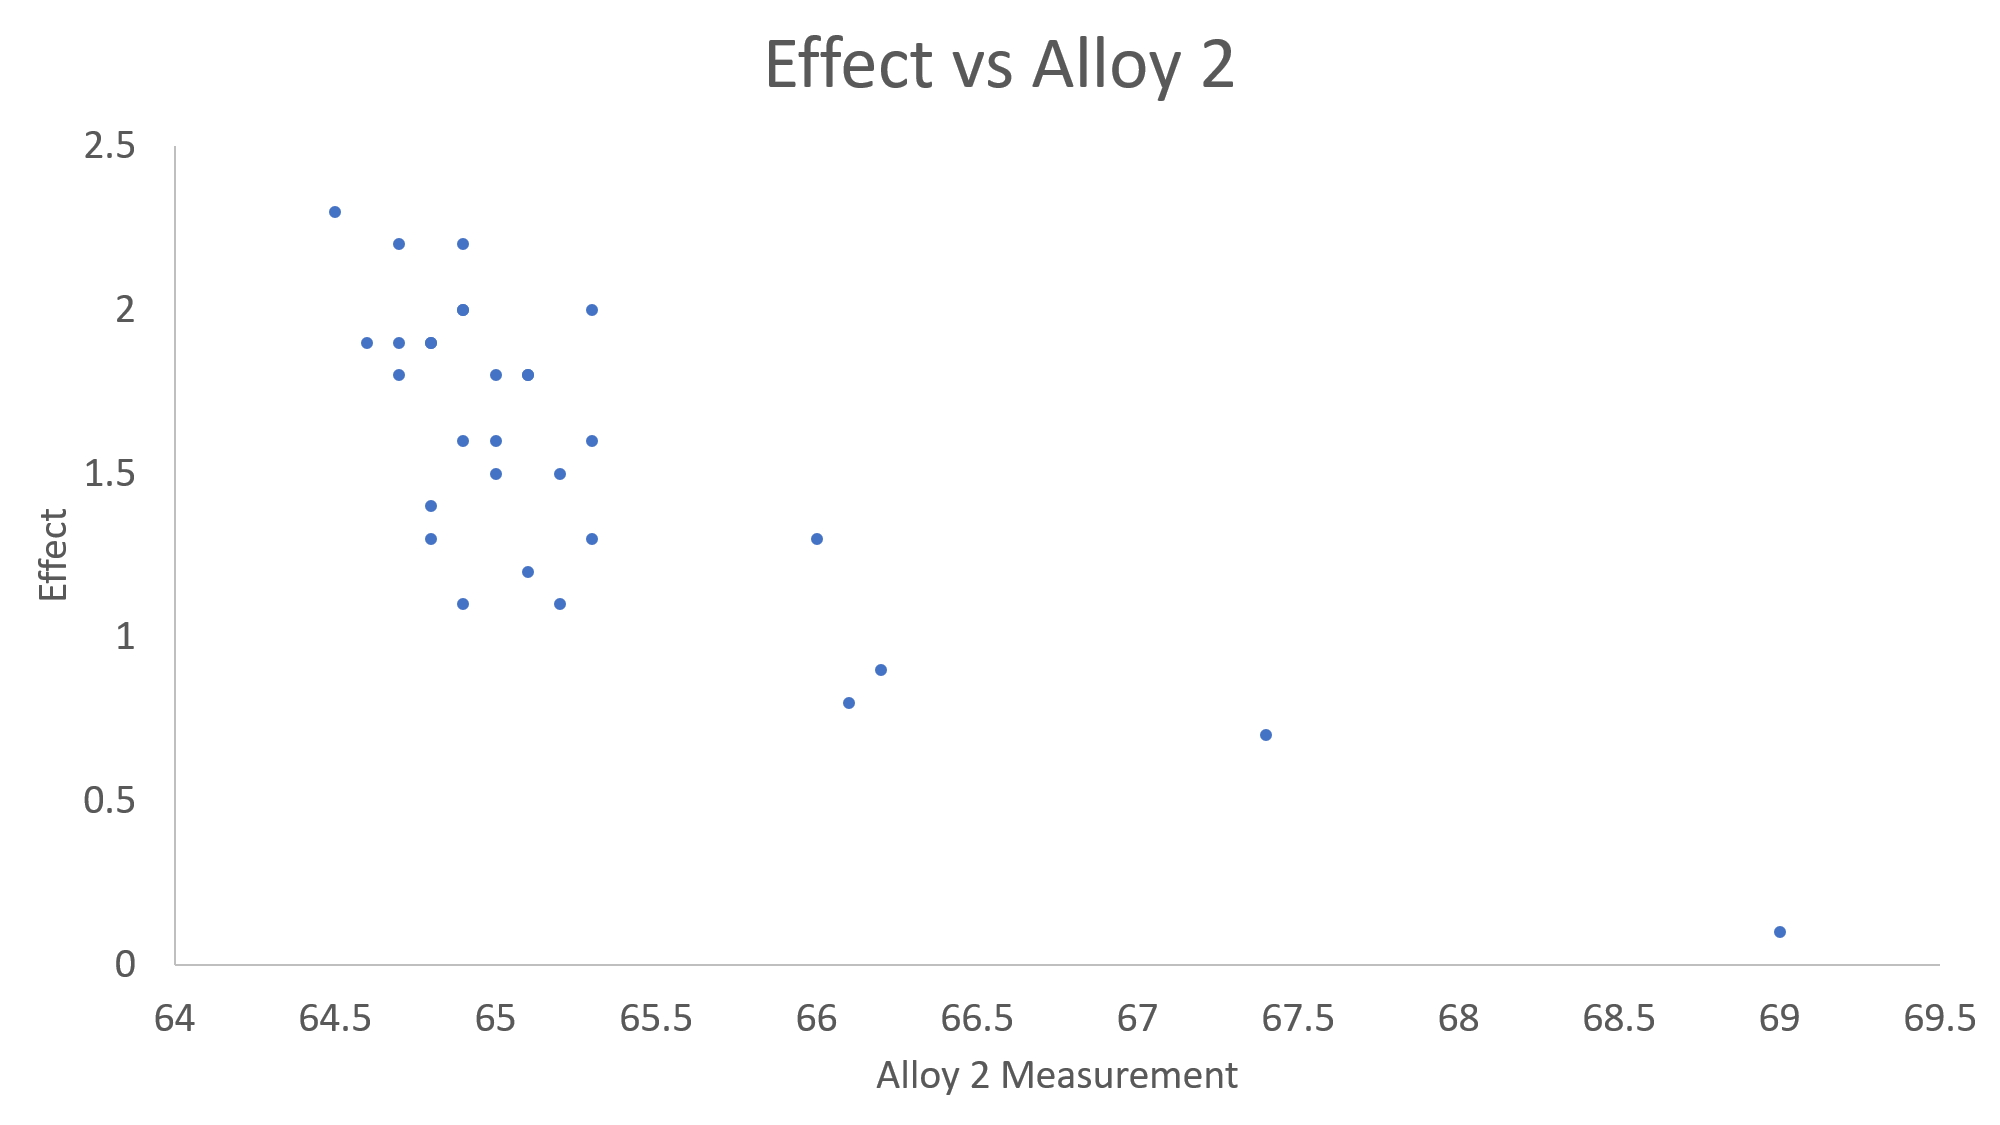
\includegraphics[width=\textwidth]{q6.png}
 \caption{My caption}
 \label{q6}
\end{figure}

From the scatterplot above, we can clearly see that with higher strength, the effect
is less. This suggests that the effect of the treatment is not independent of the initial strength of the rods. The relationship appears to be linear.

\end{document}
